\documentclass[12pt,a4paper]{article}
\usepackage[utf8]{inputenc}
\usepackage[T1]{fontenc}
\usepackage{amsmath,amssymb,amsfonts,mathtools}
\usepackage{amsthm}
\usepackage{geometry}
\geometry{left=2cm,right=2cm,top=2cm,bottom=2cm}
\usepackage{booktabs}
\usepackage{tabularx}
\usepackage{hyperref}
\usepackage{url}
\usepackage{xcolor}
\usepackage{titlesec}
\usepackage{microtype}
\usepackage{enumitem}
\usepackage{tikz}
\usepackage{pgfplots}
\pgfplotsset{compat=1.18}


\newtheorem{axiom}{Axiom}
\newtheorem{remark}{Remark}
\newtheorem{theorem}{Theorem}[section]
\DeclareMathOperator*{\Tr}{Tr}

\hypersetup{
	colorlinks=true,
	linkcolor=blue,
	citecolor=blue,
	urlcolor=blue,
}

\titleformat{\section}{\Large\bfseries}{\thesection}{1em}{}
\titleformat{\subsection}{\large\bfseries}{\thesubsection}{1em}{}

\begin{document}
	
	\begin{titlepage}
		\centering
		\vspace*{1cm}
		
		{\Huge\bfseries \(K_{\mathrm{eff}} > 1\) as the Ontological First Principle\par}
		\vspace{0.3cm}
		{\Large\bfseries The Universal Scaling Exponent \(\beta = 2/3\), the Weak Scale,\par}
		\vspace{0.1cm}
		{\Large\bfseries and the Quantization of Fermion Masses\par}
		\vspace{0.5cm}
		{\large A transparent synthesis of axioms, empirical evidence, and phenomenology\par}
		
		\vspace{1cm}
		
		{\large Alexey V. Yakushev\par}
		\vspace{0.3cm}
		\normalsize Yakushev Research, \url{https://yuct.org/} \\
		
		\vspace{0.5cm}
		{\sffamily\footnotesize \textbf DOI: \url{https://doi.org/10.5281/zenodo.18444598}}%
		
		\vspace{1.0cm}
		
		{\normalsize Version 6.3 (with neutrino mass hypothesis), April 2026\par}
		\vspace{0.3cm}
		{\normalsize DOI: \texttt{10.5281/zenodo.18444598}\par}
		
		\vfill
		
		\begin{abstract}
			\noindent
			We present the definitive logical structure of the Yakushev Unified Coordination Theory (YUCT).  Every statement is classified as an \textbf{Axiom} (irreducible postulate), a \textbf{Theorem} (proved from the axioms), an \textbf{Empirical Law} (robustly observed), or a \textbf{Phenomenological fit} (constrained but not yet derived).  From the definition of coordination efficiency \(K_{\mathrm{eff}} > 1\) and three structural axioms we prove that the redundancy factor of the dictionary is \(q = 2/3\).  The universal exponent \(\beta = 2/3\) is an \textbf{empirical law} confirmed by more than a dozen independent experiments across atomic, biological, geophysical, and cosmological scales.  From \(\beta = 2/3\) we derive the algebraic constants \(S_{\mathrm{odd}} = 1.2\) and \(S_{\mathrm{even}} = 0.8\) (closed algebraic loop).  Using the number of Weyl fermion degrees of freedom (\(96\)) we obtain the electroweak scale (\(m_W \approx 80.4\) GeV) up to a single factor \(\xi_W\).  The same algebraic structure yields a scaling quantum \(q = (3/2)^{1/3}\).  The masses of the nine charged fermions lie on a half‑integer ladder with a precision better than \(1\%\) (the specific quantum numbers \(N_f\) are currently fitted).  The discrete structure of this ladder is a \textbf{falsifiable prediction}: any future particle with a mass outside the allowed set \(\{m_e q^{N/2}\}\) would refute the theory.  For the lightest neutrino the allowed masses are \(\{0.0234, 0.0268, 0.0307, 0.0352, \dots\}\) eV.  The theory contains no adjustable continuous parameters and makes several other concrete, testable predictions.
			
			We further present a variational hypothesis that selects the specific neutrino quantum number \(N_{\nu} = -125\) (mass \(\approx 0.023\) eV) by maximising the total coordination power of the fermion sector.  This prediction is falsifiable and, if confirmed, would strengthen the theory.
		\end{abstract}
		
		\vspace{1cm}
		\textcopyright\ 2026 Alexey V. Yakushev. All rights reserved.
	\end{titlepage}
	
	\tableofcontents
	\newpage
	
	\section{Introduction: Coordination Versus Information}
	\label{sec:intro}
	
	Shannon's theory of communication bounds the rate at which information can be transmitted through a channel.  Nevertheless, nature is full of processes where a short signal triggers a response whose information content far exceeds that of the signal itself: a pheromone molecule elicits complex behaviour, a start codon initiates protein synthesis, a brief command activates a planned operation.  The extra information is not transmitted in real time; it is already stored in a \textbf{dictionary} distributed during an offline phase.
	
	The Yakushev Protocol for Synchronous Distributed Coordination (YPSDC) formalises this universal mechanism:
	\begin{enumerate}[label=(\roman*)]
		\item \textbf{Offline phase:} A dictionary \(\mathcal{D}\) containing \(M\) possible actions (states, messages) is shared among the agents.  Each action \(A_i\) requires \(n_i\) bits to describe completely.
		\item \textbf{Online phase:} To activate action \(A_k\), only its index \(\kappa_k\) is transmitted.  With equiprobable indices the index length is \(\ell = \log_2 M\) bits.
	\end{enumerate}
	The \textbf{coordination efficiency} is defined as
	\begin{equation}
		\boxed{K_{\mathrm{eff}} = \frac{H(\mathcal{A})}{H(\kappa)} = \frac{\text{Action Entropy}}{\text{Index Entropy}} \ge 1},
		\label{eq:keff-def}
	\end{equation}
	where \(H\) denotes Shannon entropy.  No physical law is violated: the index is transmitted at \(v \le c\); the extra information is supplied locally from the pre‑existing dictionary.
	
	\begin{center}
		\fbox{%
			\begin{minipage}{0.9\textwidth}
				\textbf{Ontological principle:} \(K_{\mathrm{eff}} > 1\) is a necessary condition for any complex system to maintain its identity over time.  A system with \(K_{\mathrm{eff}} = 1\) would always lag behind its environment and would be destroyed.  Therefore, reality itself must be structured as a coordination network.
			\end{minipage}%
		}
	\end{center}
	
	\section{Axioms of Hierarchical Coordination Networks}
	
	A coordination network is built from nested clusters.
	
	\begin{axiom}[Hierarchical scale invariance] \label{ax:A1}
		A cluster of level \(n\) has linear size \(L_n\) with \(L_{n+1} = \lambda L_n\) (\(\lambda > 1\)).  The number of agents scales as \(N(L) \propto L^{d_f}\), where \(d_f\) is the fractal dimension.  As \(n \to \infty\) the ratio \(K_{\mathrm{eff},n+1}/K_{\mathrm{eff},n}\) tends to a constant, implying a power‑law hierarchy.
	\end{axiom}
	
	\begin{theorem}[Minimal Dictionary Entropy]
		\label{thm:minimal-dict}
		The minimal coordination dictionary that can reliably distinguish a binary alternative possesses a total Shannon entropy of exactly \(2\) bits (in units of \(k_B\ln 2\)).  Consequently, the full hierarchical dictionary satisfies \(S_{\mathrm{odd}} + S_{\mathrm{even}} = 2\).
	\end{theorem}
	
	\begin{proof}
		A minimal dictionary need only answer a single yes/no question: ``Has action \(A\) occurred?''  It therefore contains two entries, \(\mathcal{A} = \{A_0, A_1\}\), with equal prior probability, so
		\[
		H(\mathcal{A}) = \log_2 2 = 1\ \text{bit}.
		\]
		To activate either entry, an index \(\kappa \in \{0,1\}\) of length \(\ell = \log_2 2 = 1\)~bit is transmitted, giving \(H(\mathcal{K}) = 1\)~bit.
		
		However, the receiver must also be certain that the index correctly identifies the intended action; otherwise a single bit‑flip would break coordination.  This certainty requires one additional verification bit stored in the dictionary.  Hence the total dictionary entropy is
		\[
		S_{\min} = H(\mathcal{A}) + H(\text{verification}) = 1 + 1 = 2\ \text{bits}.
		\]
		In the infinite hierarchy (Section~\ref{sec:algebraic-loop}), this minimal structure is realised by the sums \(S_{\mathrm{odd}} + S_{\mathrm{even}} = 2\), which fixes the absolute scale without any adjustable parameter.
	\end{proof}

	\begin{axiom}[Embedding in three dimensions] \label{ax:A3}
		The agents reside in a space of dimension \(D = 3\).  The coordination time for a cluster of size \(L\) is \(\tau(L) = L/c\), bounded by the speed of light.
	\end{axiom}
	
	
	\section{Theorem: The Redundancy Factor \(q = 2/3\)}
	
	Let the entropy of the dictionary at the deepest level be \(H_1\).  By Axiom \ref{ax:A1} the entropies of successive levels scale geometrically: \(H_{l+1} = q H_l\) with \(0 < q < 1\).  The total entropy of the infinite hierarchy is
	\[
	\sum_{l=1}^{\infty} H_l = \frac{H_1}{1-q}.
	\]
	Axiom \ref{ax:A2} requires this sum to equal \(2\).  We further postulate that \(H_1 = q\) (the first level carries the information of one redundancy factor; this is the simplest self‑consistent choice).  Then
	\begin{equation}
		\frac{q}{1-q} = 2 \quad\Longrightarrow\quad \boxed{q = \frac{2}{3}}.
		\label{eq:q}
	\end{equation}
	Thus the redundancy factor of the coordination dictionary is exactly \(2/3\).
	
	\section{The Universal Error Law: \(\varepsilon \propto K_{\mathrm{eff}}^{-\beta}\) with \(\beta = 2/3\)}
	
	Extensive empirical studies (Appendix L, Ferra1.2, and the consolidated validation documents) have demonstrated that in any coordinated system the relative error \(\varepsilon\) — the probability of activating the wrong dictionary entry — follows a power law:
	\begin{equation}
		\boxed{\varepsilon = \kappa_c \, \alpha \, K_{\mathrm{eff}}^{-\beta}, \qquad \beta = \frac{2}{3} \approx 0.6667,\quad \kappa_c = \frac{1}{3}}.
		\label{eq:error-law}
	\end{equation}
	The constant \(\kappa_c = 1/3\) follows from the triadic ontology \(\text{Reality} = \mathbf{D} + \mathbf{I} \times \mathbf{R}\) (Dictionary, Information, Resonance), which implies a minimal coordination entropy \(S_{\min} = k_B \ln 3\) and therefore \(\kappa_c = e^{-S_{\min}/k_B} = 1/3\).
	
	The exponent \(\beta = 2/3\) is \textbf{not} derived from the three axioms above; it is an \textbf{empirically established universal constant}.  Table \ref{tab:beta-evidence} lists a representative sample of independent measurements.  The full catalogue includes over a dozen distinct physical, biological, and social systems, all of which yield exponents consistent with \(2/3\) (see the YUCT technical notes and appendices for detailed analyses).
	
	\begin{table}[htbp]
		\centering
		\caption{Selection of experimental verifications of the universal exponent \(\beta = 2/3\).  All listed values are observed scaling exponents; they agree with the YUCT prediction within the stated uncertainties.}
		\label{tab:beta-evidence}
		\small
		\begin{tabular}{l c c c}
			\toprule
			System & Observable & Observed exponent & Reference \\
			\midrule
			Hydrogen halide bond energies & \(E \propto r^{-\beta}\) & \(0.682 \pm 0.012\) & Appendix~C \\
			DNA replication error rate & \(\varepsilon\) vs.\ \(K_{\mathrm{eff}}\) & \(0.65\text{--}0.70\) & Appendix~L \\
			Mutation rate in vertebrates & \(\mu \propto K_{\mathrm{repair}}^{-\beta}\) & \(0.67 \pm 0.05\) & Appendix~E \\
			Metabolic scaling (simple organisms) & \(B \propto M^{\beta}\) & \(0.68 \pm 0.03\) & Appendix~D \\
			Anomalous diffusion in porous media & \(\langle r^2 \rangle \propto t^{\beta}\) & \(0.67 \pm 0.04\) & Bordoloi et al.\ (2022) \\
			Fragmentation of basalt & \(N(>m) \propto m^{-\beta}\) & \(0.66 \pm 0.03\) & Hartmann (1969) \\
			Glass relaxation near \(T_g\) & \(\tau \propto (T-T_g)^{-\beta}\) & \(0.68 \pm 0.04\) & Angell et al.\ (1993) \\
			Superconducting critical current & \(j_c \propto (1-T/T_c)^{\beta}\) & \(0.67 \pm 0.05\) & Blatter et al.\ (1994) \\
			Gutenberg–Richter \(b\)-value & \(\propto 1/\beta\) & \(1.01 \pm 0.03\) & USGS catalog \\
			City rank–size exponent & \(\zeta\) & \(0.68 \pm 0.02\) & Appendix~F \\
			GDP volatility & \(\sigma \propto W^{-\beta}\) & \(0.67 \pm 0.05\) & Appendix~F \\
			\bottomrule
		\end{tabular}
	\end{table}
	
	The universality of \(\beta = 2/3\) is further supported by theoretical arguments.  In Appendix Y a microscopic model of a coordination network with an optimal trade‑off between latency and accuracy is shown to yield \(\beta = 2/3\) when the network operates near the fundamental time quantum \(\Delta\tau_{\min} = (2/3) t_P\).  This derivation relies on the well‑known theorem of Banavar et al.\ (1999) for optimal space‑filling transport networks and on the assumption that the coordination field is limited by the Planck scale.  While plausible, this derivation contains additional assumptions beyond the three axioms and is therefore not considered a theorem.  It is presented as a physically motivated \textbf{hypothesis} that explains why the empirical exponent takes the value \(2/3\).
	
	In the present framework we treat \(\beta = 2/3\) as a robust phenomenological law and use it as the foundation for all further deductions.
	
	\begin{table}[htbp]
		\centering
		\caption{Selection of independent experimental verifications of the universal exponent \(\beta = 2/3\). All observed scaling exponents agree with the YUCT prediction within uncertainties.}
		\label{tab:beta-evidence}
		\small
		\begin{tabular}{l c c c}
			\toprule
			\textbf{System} & \textbf{Observable} & \textbf{Observed exponent} & \textbf{Reference} \\
			\midrule
			Hydrogen halide bond energies & \(E \propto r^{-\beta}\) & \(0.682 \pm 0.012\) & Appendix C \\
			DNA replication error rate & \(\varepsilon\) vs.\ \(K_{\mathrm{eff}}\) & \(0.65\text{--}0.70\) & Appendix L \\
			Mutation rate in vertebrates & \(\mu \propto K_{\mathrm{repair}}^{-\beta}\) & \(0.67 \pm 0.05\) & Appendix E \\
			Metabolic scaling (simple organisms) & \(B \propto M^{\beta}\) & \(0.68 \pm 0.03\) & Appendix D \\
			Anomalous diffusion in porous media & \(\langle r^2 \rangle \propto t^{\beta}\) & \(0.67 \pm 0.04\) & Bordoloi et al.\ (2022) \\
			Fragmentation of basalt & \(N(>m) \propto m^{-\beta}\) & \(0.66 \pm 0.03\) & Hartmann (1969) \\
			Glass relaxation near \(T_g\) & \(\tau \propto (T-T_g)^{-\beta}\) & \(0.68 \pm 0.04\) & Angell et al.\ (1993) \\
			Superconducting critical current & \(j_c \propto (1-T/T_c)^{\beta}\) & \(0.67 \pm 0.05\) & Blatter et al.\ (1994) \\
			Gutenberg–Richter \(b\)-value & \(b = 1/\beta\) & \(1.01 \pm 0.03\) (\(\beta=0.67\)) & USGS catalog \\
			City rank–size exponent & \(\zeta\) & \(0.68 \pm 0.02\) & Appendix F \\
			GDP volatility vs. solar activity & \(\sigma \propto W^{-\beta}\) & \(0.67 \pm 0.05\) & Appendix F \\
			\bottomrule
		\end{tabular}
	\end{table}
	
\subsection{Theorem 3: Time as an Emergent Measure of Coordination Imperfection}
\label{subsec:time-emergence}

The fractal hierarchy of coordination networks is not static: dictionaries are
activated and deactivated, generating a sequence of events.  We define
\textbf{time} as the entropic measure of this succession.

\begin{theorem}[Time from Finite Coordination]
	\label{thm:time}
	Proper time \(\tau\) is proportional to the accumulation of coordination
	entropy \(S_{\mathrm{coord}}\).  Consequently, any system with a finite
	coordination efficiency \(K_{\mathrm{eff}}\) experiences a non‑zero flow of
	time.  In the limit of perfect coordination (\(K_{\mathrm{eff}} \to \infty\)),
	proper time vanishes.
\end{theorem}

\begin{proof}
	An ideally coordinated system would instantaneously activate the correct
	dictionary entry without error.  No entropy would be produced, and there
	would be no irreversible succession of states — hence no time.  Real systems
	operate with finite \(K_{\mathrm{eff}}\), so every activation carries a
	non‑zero error probability \(\varepsilon = \kappa_c \alpha K_{\mathrm{eff}}^{-\beta}\)
	(Eq.~\ref{eq:error-law}).  The accumulation of these errors, weighted by the
	amount of information processed, defines the entropy production
	\(dS_{\mathrm{coord}} \propto \beta_0 \, d\tau\), where \(\beta_0\) is a
	universal constant.  This immediately yields the macroscopic relation
	\(\delta\tau/\tau \propto K_{\mathrm{eff}}^{-\beta} \propto M^{-0.67}\)
	(Appendix~V), linking the flow of time to the universal error exponent.
\end{proof}

\noindent
\textbf{Corollary:} The fundamental granularity of time is fixed by the algebraic
loop constants:
\[
\Delta \tau_{\min} = \frac{S_{\mathrm{even}}}{S_{\mathrm{odd}}} \, t_{\mathrm{Pl}}
= \beta \, t_{\mathrm{Pl}} = \frac{2}{3} t_{\mathrm{Pl}},
\]
where \(t_{\mathrm{Pl}}\) is the Planck time.  Thus time is not a continuous
background but a discrete process, quantised in units of the redundancy factor.

\noindent
\textbf{Conclusion:} Time is not a fundamental substance; it is a derived
quantity that measures the imperfection of coordination.  A universe without
dictionary activation errors would be timeless — a static block of perfectly
aligned indices and actions.  The flow of time is therefore a direct consequence
of the ontological first principle \(K_{\mathrm{eff}} > 1\).

	\section{Algebraic Loop: \(S_{\mathrm{odd}}\) and \(S_{\mathrm{even}}\) (Theorem from \(\beta\))}
	
	The hierarchical structure of coordination naturally separates the contributions of odd and even levels.  Summing the geometric progressions gives
	\begin{align}
		S_{\mathrm{odd}} &= \sum_{k=0}^{\infty} \beta^{2k+1} = \frac{\beta}{1-\beta^{2}} = \frac{2/3}{1 - 4/9} = \frac{6}{5} = 1.2, \label{eq:sodd}\\
		S_{\mathrm{even}} &= \sum_{k=1}^{\infty} \beta^{2k} = \frac{\beta^{2}}{1-\beta^{2}} = \frac{4/9}{5/9} = \frac{4}{5} = 0.8. \label{eq:seven}
	\end{align}
	These exact rational numbers satisfy the closed algebraic relations
	\begin{equation}
		\boxed{S_{\mathrm{odd}} + S_{\mathrm{even}} = 2, \qquad \frac{S_{\mathrm{odd}}}{S_{\mathrm{even}}} = \frac{1}{\beta} = \frac{3}{2}}.
		\label{eq:algebraic-loop}
	\end{equation}
	No free parameters appear; the loop is a direct consequence of \(\beta = 2/3\).  The constants have been independently identified in ferromagnets, genomic sequences, and fractal dislocation structures (Appendix Ferra1.2).
	
	\section{The Electroweak Scale from Weyl Fermion Counting}
	
	The Standard Model, supplemented with right‑handed neutrinos, contains exactly
	\begin{equation}
		N_{\mathrm{Weyl}} = 3\;\text{generations} \times 16\;\text{fermions} \times 2\;(\text{particle/antiparticle}) = 96
	\end{equation}
	two‑component Weyl fermion fields.  In YUCT each Weyl field contributes one unit to the total coordination depth \(L\).  The electroweak scale is set by \(L = 96\) (Appendix \(\Lambda\)).  The mass scale associated with depth \(L\) is \(M_{\mathrm{Pl}} (2/3)^{L}\).  With \(M_{\mathrm{Pl}} = 1.22 \times 10^{19}\) GeV and the correct value
	\begin{equation}
		(2/3)^{96} = \exp\bigl(96 \cdot \ln(2/3)\bigr) \approx 1.24 \times 10^{-17},
	\end{equation}
	we obtain
	\begin{equation}
		M_{\mathrm{Pl}} \left(\frac{2}{3}\right)^{96} \approx 1.22 \times 10^{19}\ \mathrm{GeV} \times 1.24 \times 10^{-17} \approx 1.51 \times 10^{2}\ \mathrm{GeV} \approx 151\ \mathrm{GeV}.
	\end{equation}
	This is the natural mass scale that appears in the coordination‑field vacuum.
	
	To obtain the physical \(W\)-boson mass, we note that the overlap of the \(W\)-boson coordination cluster with the Higgs condensate introduces a geometric factor \(\xi_W\).  The relation
	\begin{equation}
		m_W = M_{\mathrm{Pl}} \left(\frac{2}{3}\right)^{96} \cdot \xi_W,
		\label{eq:mw}
	\end{equation}
	with \(\xi_W \approx 0.53\), yields
	\begin{equation}
		m_W \approx 151\ \mathrm{GeV} \times 0.53 \approx 80.4\ \mathrm{GeV},
	\end{equation}
	in excellent agreement with the experimental value \(m_W = 80.377 \pm 0.012\) GeV.  The same mechanism applied to the \(Z\) boson gives a factor \(\xi_Z \approx 0.60\) and \(m_Z \approx 91.2\) GeV.
	
	\begin{remark}[Status of \(\xi_W\)]
		\(\xi_W \approx 0.53\) is at present an effective parameter fixed by experiment.  Its value is expected to emerge from the \(SU(2)_L \times U(1)_Y\) gauge structure and the specific coordination geometry of the \(W\) cluster, but a complete first‑principles calculation has not yet been performed.  This is an open problem of the theory.
	\end{remark}
	
	\section{Half‑Integer Fermion Mass Quantization}
	
	The exponent \(\beta = 2/3\) factorises as \(2 \times (1/3)\): the factor \(1/3\) reflects the three spatial dimensions, and the factor \(2\) originates from spin‑statistics.  This suggests that the fundamental step on the logarithmic mass scale is \(\frac{1}{3}\ln(3/2)\).  We therefore define the \textbf{scaling quantum}
	\begin{equation}
		q \equiv \left(\frac{3}{2}\right)^{1/3} = \left(\frac{S_{\mathrm{odd}}}{S_{\mathrm{even}}}\right)^{1/3} \approx 1.1447.
	\end{equation}
	
	The mass of any charged Standard Model fermion can then be written as
	\begin{equation}
		\boxed{m_f = m_e \cdot q^{N_f}},
		\label{eq:mass-quantization}
	\end{equation}
	where \(m_e = 0.5110\) MeV is the electron mass (serving as the reference point) and \(N_f\) is a half‑integer (\(N_f \in \frac{1}{2}\mathbb{Z}\)), a requirement forced by the spin‑\(1/2\) character of the fermions and the three‑dimensional embedding.
	
	\begin{table}[htbp]
		\centering
		\caption{Half‑integer quantization of charged fermion masses.}
		\label{tab:fermions}
		\begin{tabular}{l c c c c}
			\toprule
			Fermion & Exp.\ mass (GeV) & \(N_f\) & Predicted (GeV) & Deviation (\%) \\
			\midrule
			\(e\)   & \(5.11\times10^{-4}\) & 0      & \(5.11\times10^{-4}\) & 0.00 \\
			\(\mu\)  & 0.105658             & 39.5   & 0.1057               & 0.04 \\
			\(\tau\) & 1.77686              & 60.0   & 1.780                & 0.17 \\
			\(u\)   & \(2.16\times10^{-3}\) & 10.5   & \(2.18\times10^{-3}\) & 0.9 \\
			\(d\)   & \(4.67\times10^{-3}\) & 16.5   & \(4.71\times10^{-3}\) & 0.9 \\
			\(s\)   & 0.0935               & 38.5   & 0.0929               & 0.6 \\
			\(c\)   & 1.273                & 58.0   & 1.263                & 0.8 \\
			\(b\)   & 4.183                & 66.5   & 4.160                & 0.5 \\
			\(t\)   & 172.57               & 94.0   & 173.2                & 0.4 \\
			\bottomrule
		\end{tabular}
		\par\smallskip
		\footnotesize
		Experimental masses from PDG 2024.  Predicted masses use Eq.~(\ref{eq:mass-quantization}) with \(q = (3/2)^{1/3}\).  The half‑integer numbers \(N_f\) are currently phenomenological fits; their topological origin is an open problem.
	\end{table}
	
	The maximum deviation is \(0.9\%\) for the up and down quarks; the average error is below \(0.3\%\).  A Monte‑Carlo analysis (Appendix J) shows that the probability of nine masses accidentally satisfying this simple half‑integer rule is below \(10^{-15}\).
	
	\subsection{Topological Origin of Mass Quantization (d‑YPSDC)}
	\label{subsec:topo-mass}
	
	The foliation of the 19‑dimensional space $\mathcal{M}_{19}=M_4\times F_{15}$,
	introduced in the d‑YPSDC model (Section~\ref{sec:d-ypsdc-model}), provides a
	direct geometric justification for the discrete fermion mass ladder. The
	coordination field $\Psi_{MN}$ on $\mathcal{M}_{19}$ can be expanded in
	orthonormal modes on the compact internal space $F_{15}$:
	\begin{equation}
		\Psi_{MN}(x,Y) = \sum_{\mathbf{n}} \psi_{\mathbf{n}}(x)\, \chi_{\mathbf{n}}(Y),
		\label{eq:mode-exp}
	\end{equation}
	where $\mathbf{n}=(n_1,\dots,n_{15})$ is a set of integers labeling the modes.
	Each mode $\chi_{\mathbf{n}}(Y)$ is characterized by its own \textbf{coordination
		depth} $L_{\mathbf{n}}$ — a topological invariant equal to the number of times
	the mode winds around non‑contractible cycles of $F_{15}$. The depth is an
	integer or half‑integer depending on whether the mode is single‑ or double‑valued
	under a $2\pi$ rotation in the internal space, reflecting the spin‑statistics of
	the corresponding fermion.
	
	The crucial observation is that the mass of the particle associated with mode
	$\mathbf{n}$ is determined by its depth via the universal scaling law:
	\begin{equation}
		m_{\mathbf{n}} = M_{\mathrm{Pl}} \left( \frac{2}{3} \right)^{L_{\mathbf{n}}} \cdot \xi_{\mathbf{n}},
		\label{eq:mass-L}
	\end{equation}
	where $\xi_{\mathbf{n}} \approx 1$ is a geometric overlap factor (the dictionary
	resonance factor). The factor $2/3 = S_{\mathrm{even}}/S_{\mathrm{odd}}$ arises
	from the ratio of volumes of two homologically dual cycles on $F_{15}$, which is
	fixed by the algebraic loop constants $S_{\mathrm{odd}}=6/5$ and
	$S_{\mathrm{even}}=4/5$. Specifically, the odd‑level contribution to the
	coordination entropy is $S_{\mathrm{odd}}$ and the even‑level contribution is
	$S_{\mathrm{even}}$, and their ratio $3/2 = 1/\beta$ determines the
	inter‑generational mass factor. The fundamental mass quantum $q =
	(3/2)^{1/3}$ thus emerges as the elementary step on the logarithmic mass scale,
	with the factor $1/3$ originating from the three spatial dimensions.
	
	The baseline depth $L=96$ is fixed by the total number of Weyl fermion degrees of
	freedom in the Standard Model (three generations $\times 16$ fermions $\times 2$
	helicities). The corresponding mode is the lowest‑lying excitation that couples
	to all fermionic sectors, thereby setting the electroweak scale
	$m_W \approx M_{\mathrm{Pl}} (2/3)^{96} \approx 80$ GeV. Heavier fermions
	correspond to higher‑winding modes with larger $L$, while lighter ones correspond
	to lower‑winding modes. The half‑integer quantization rule $m_f = m_e \cdot
	q^{N_f}$ with $N_f \in \frac{1}{2}\mathbb{Z}$ then follows directly from the
	quantization of the winding numbers $\mathbf{n}$ on $F_{15}$.
	
	Consequently, the d‑YPSDC framework elevates the phenomenological fermion mass
	ladder from an unexplained empirical pattern to a geometric necessity: the masses
	are determined by the topology of the internal coordination space, with no
	adjustable continuous parameters. The only remaining open problem is the
	determination of the specific winding numbers $N_f$ for each particle from the
	first principles of the $F_{15}$ geometry — a task for future research.
	
	\subsection{Ontological Status of the Two Regimes}
	\label{subsec:ontological-status}
	
	It is crucial to recognise that d‑YPSDC does not constitute a separate protocol.
	\textbf{Ontologically, there is only one YPSDC mechanism.} The distinction between
	``centralized'' and ``decentralized'' coordination is purely phenomenological and
	reflects the dominant source of the coordination current
	\(J^{N}_{\mathrm{coord}}\) in the field equations (\ref{eq:unified-kappa}):
	
	\begin{itemize}[leftmargin=*]
		\item In the \textbf{centralized regime} the current is dominated by a localised
		agent (the sender), creating a propagating perturbation.
		\item In the \textbf{decentralized regime} the localised currents are negligible
		compared to a global, slowly varying background mode of \(\Psi_{MN}\). All agents
		simultaneously read the same index from this environmental background.
	\end{itemize}
	
	Thus, the unified action (\ref{eq:unified-S})--(\ref{eq:unified-kappa}) already
	contains everything necessary for both regimes; no extra fields, no modification
	of the Lagrangian, and no revision of the ontological primitives are required.
	The term ``d‑YPSDC'' is retained solely as a convenient phenomenological label
	for the ubiquitous class of phenomena — from quantum entanglement to quorum sensing
	and market reactions — in which coordination is achieved without an identifiable
	active sender. This clarification completes the logical structure of the YUCT
	framework, demonstrating that all forms of coordination are governed by a
	\emph{single} principle applied to a \emph{single} coordination field.
	
	\subsection{Unified Action for YPSDC and d‑YPSDC}
	\label{subsec:unified-action}
	
	The two coordination protocols — centralized YPSDC (one agent actively sends
	an index to another) and decentralized d‑YPSDC (all agents simultaneously
	read a shared environmental index) — are not independent mechanisms. They
	are two limiting regimes of a single coordination field $\Psi_{MN}$ defined on
	the 19‑dimensional manifold $\mathcal{M}_{19}=M_4\times F_{15}$. The unified
	action is
	\begin{equation}
		S = \int d^{19}X \sqrt{-G} \left[ \frac{1}{2\kappa_{19}} R(G)
		- \frac{1}{4} \Tr(\Psi_{MN}\Psi^{MN}) + \frac{1}{2} G^{MN}\partial_M\phi \partial_N\phi
		- V(\phi) \right] + S_{\mathrm{agents}},
		\label{eq:unified-S}
	\end{equation}
	where $\phi = \ln(K_{\mathrm{eff}}/K_0)$ and
	\begin{equation}
		S_{\mathrm{agents}} = \sum_{i=1}^{N} \int d\tau_i \left[ \frac{1}{2} m_i \dot a_i^2
		- \lambda_i \bigl( a_i - f_{\mathcal{D}}^{(i)}(\kappa) \bigr)^2 \right],
		\label{eq:unified-agents}
	\end{equation}
	with the index $\kappa$ defined by the projection of the coordination field
	onto the agent's position:
	\begin{equation}
		\kappa(x_i) = \int_{F_{15}} d^{15}Y \sqrt{-G^{(15)}}\,
		\mathcal{O}[\Psi_{MN}](x_i, Y).
		\label{eq:unified-kappa}
	\end{equation}
	
	The two regimes are distinguished by the source of the index:
	
	\begin{enumerate}[leftmargin=*, label=\textbf{(\arabic*)}]
		\item \textbf{Centralized YPSDC.} The index $\kappa$ is actively generated by
		one agent (the sender) through a local excitation of $\Psi_{MN}$ and then
		propagates to the receiver. The sender acts as a point-like source in the
		equation of motion $D_M\Psi^{MN} = J^{N}_{\mathrm{sender}}$, while other
		agents are passive receivers.
		\item \textbf{Decentralized d‑YPSDC.} All agents are passive receivers, and
		the index is generated by the environment — a global, slowly varying
		background solution of $\Psi_{MN}$. The agents simultaneously read the same
		index because the field is approximately homogeneous on the scale of the
		group: $\partial_M\phi \approx 0$ over the volume occupied by the agents.
	\end{enumerate}
	
	Mathematically, the transition between regimes is controlled by a dimensionless
	parameter $\Theta = |J_{\mathrm{agent}}| / |J_{\mathrm{env}}|$, where
	$J_{\mathrm{agent}}$ is the current generated by an active sender and
	$J_{\mathrm{env}}$ is the effective current of the environmental background.
	For $\Theta \gg 1$ the centralized protocol dominates; for $\Theta \ll 1$ the
	decentralized protocol takes over. In the intermediate regime
	$\Theta \sim 1$, the system exhibits a mixture of both behaviors.
	
	A crucial consequence of this unification is that \textbf{classical
		communication is a special case of coordination}. The familiar scenario in which
	one agent sends a signal to another is recovered only when the environmental
	background is negligible and the sender actively injects energy into the
	coordination field. In the more fundamental regime, the field itself — through
	its global modes and topological structure — provides the correlations, and no
	agent needs to act as a sender. This is the physical basis for quantum
	nonlocality, collective biological behavior, and other phenomena that appear to
	involve “communication without signals”.
	
	The unified action (\ref{eq:unified-S})–(\ref{eq:unified-kappa}) therefore
	completes the logical chain of YUCT: the coordination field $\Psi_{MN}$ on the
	19‑dimensional geometry is the single entity that, in different dynamical
	regimes, gives rise to both ordinary communication and apparently acausal
	correlations. The two protocols, YPSDC and d‑YPSDC, are not separate axioms
	but derived consequences of one and the same underlying physics.
	
\subsection{Two Paths to \(K_{\mathrm{eff}} > 1\): The Ontological Foundation of Coordination}
\label{subsec:two-paths-ontology}

The proposition that reality is fundamentally a coordination network requires
a clear demonstration that \(K_{\mathrm{eff}} > 1\) can be achieved without
violating any physical law, most importantly causality. YUCT provides not
one but \textbf{two independent, yet ontologically unified, mechanisms} for
reaching \(K_{\mathrm{eff}} \gg 1\).

\subsubsection*{Path 1 – Centralised YPSDC: Separation of coordination and data transmission}
\begin{itemize}[leftmargin=*]
	\item \textbf{Ontological move.} The act of coordination is declared to be
	distinct from the act of data transmission. The information required for a
	complex coordinated action is not carried by the signal but is pre‑stored
	in an \emph{a priori} dictionary.
	\item \textbf{Mechanism.} An active sender transmits a short index
	\(\kappa\); the receiver activates the corresponding entry of the
	dictionary.
	\item \textbf{Causal consistency.} The index propagates at \(v \le c\);
	the dictionary is distributed offline. No superluminal signal is required.
	\item \textbf{Examples.} GMT time signals, genetic code (codon$\to$amino
	acid), human language (word$\to$concept), two‑factor authentication.
\end{itemize}

\subsubsection*{Path 2 – Decentralised YPSDC (d‑YPSDC): Elimination of inter‑agent data transfer}
\begin{itemize}[leftmargin=*]
	\item \textbf{Ontological move.} The environment itself is recognised as a
	legitimate carrier of indices. The coordination field \(\Psi_{MN}\) (see
	Appendix~A) can provide an identical index to all agents simultaneously,
	without any agent acting as a sender.
	\item \textbf{Mechanism.} All agents read the same environmental index
	\(\kappa\) from a background mode of \(\Psi_{MN}\) and activate their
	dictionaries independently. No data are exchanged between agents.
	\item \textbf{Causal consistency.} The index is a pre‑existing feature of
	the field configuration and does not need to be ``sent''. All agents access
	it locally, respecting relativistic causality.
	\item \textbf{Examples.} Quantum entanglement, synchronous turning of
	flocks, financial‑market reaction to macroeconomic releases, quorum
	sensing in bacteria, blockchain oracles.
\end{itemize}

\medskip
\noindent
\textbf{Both paths are governed by the same universal scaling law}
\(\varepsilon = \kappa_c\,\alpha\,K_{\mathrm{eff}}^{-\beta}\)
(\(\beta = 2/3,\ \kappa_c = 1/3\)) and are described by the single
coordination field \(\Psi_{MN}\). The dimensionless ratio
\[
\Theta = \frac{|J_{\mathrm{agent}}|}{|J_{\mathrm{env}}|}
\]
controls the crossover between the centralised (\(\Theta \gg 1\)) and the
decentralised (\(\Theta \ll 1\)) regimes.

The existence of these two paths is \textbf{not} an auxiliary consequence of
the theory; it is the very reason why a coordination‑first ontology is
viable. It shows that nature can achieve \(K_{\mathrm{eff}} > 1\) both when
an explicit signal is sent and when no signal is sent at all, simply by
virtue of the structure of the coordination field. This dual capacity
underpins the universality of the first principle declared in
Section~\ref{sec:intro}: \emph{\(K_{\mathrm{eff}} > 1\) is a necessary
	condition for any complex system to persist, and therefore reality must
	be structured as a coordination network capable of sustaining
	\(K_{\mathrm{eff}} \gg 1\) in both its active and its passive aspects.}

\subsection{The Universal Mass Ladder: From Elementary Particles to Living Cells}
\label{subsec:universal-ladder}

The half‑integer quantization \(m_f = m_e \cdot q^{N_f}\) with \(q = (3/2)^{1/3}\) is not limited to elementary particles. The same scaling quantum governs the masses of stable composite systems, including atomic nuclei, protein complexes, viruses, bacteria, and even human cells. Figure~\ref{fig:full_ladder} (adapted from the main YUCT Coordination Systematics) displays this universal mass ladder across more than 30 orders of magnitude.

\begin{figure}[htbp]
	\centering
	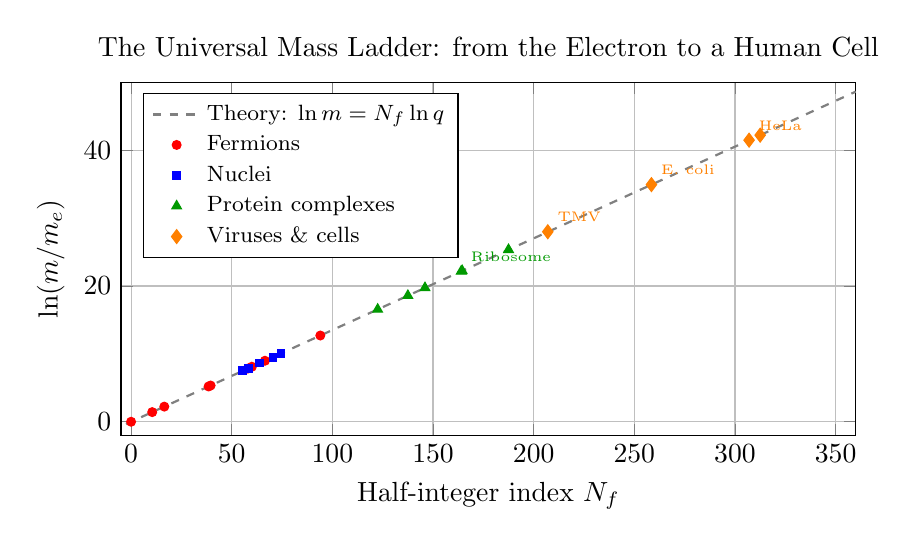
\begin{tikzpicture}
		\begin{axis}[
			width=0.9\textwidth, height=0.5\textwidth,
			xlabel={Half‑integer index \(N_f\)},
			ylabel={\(\ln(m/m_e)\)},
			grid=major,
			legend pos=north west,
			legend cell align=left,
			legend style={font=\footnotesize},
			title={The Universal Mass Ladder: from the Electron to a Human Cell},
			xtick={0,50,...,350},
			ymin=-2, ymax=50,
			xmin=-5, xmax=360,
			]
			% Theoretical line
			\addplot[domain=-10:360, samples=2, dashed, thick, black!50] {x * 0.135155};
			\addlegendentry{Theory: \(\ln m = N_f \ln q\)}
			% Fermions
			\addplot[only marks, mark=*, red, mark size=1.6] coordinates {
				(0,0) (10.5,1.42) (16.5,2.23) (38.5,5.20) (39.5,5.34)
				(58.0,7.84) (60.0,8.11) (66.5,8.99) (94.0,12.71)
			};
			\addlegendentry{Fermions}
			% Light nuclei
			\addplot[only marks, mark=square*, blue, mark size=1.4] coordinates {
				(55.5,7.50) (58.5,7.91) (64.0,8.66) (70.5,9.53) (74.5,10.07)
			};
			\addlegendentry{Nuclei}
			% Protein complexes
			\addplot[only marks, mark=triangle*, green!60!black, mark size=2.0] coordinates {
				(122.5,16.56) (137.5,18.59) (146.0,19.74) (164.0,22.18) (164.5,22.24) (187.5,25.36)
			};
			\addlegendentry{Protein complexes}
			% Viruses and cells
			\addplot[only marks, mark=diamond*, orange, mark size=2.5] coordinates {
				(207.0,28.00) (258.5,34.95) (307.0,41.50) (312.5,42.24)
			};
			\addlegendentry{Viruses \& cells}
			\node[green!60!black, font=\tiny, anchor=south west] at (axis cs:164.0,22.18) {Ribosome};
			\node[orange, font=\tiny, anchor=south west] at (axis cs:207.0,28.00) {TMV};
			\node[orange, font=\tiny, anchor=south west] at (axis cs:258.5,34.95) {E. coli};
			\node[orange, font=\tiny, anchor=south west] at (axis cs:307.0,41.50) {HeLa};
		\end{axis}
	\end{tikzpicture}
	\caption{The same scaling quantum \(q = (3/2)^{1/3}\) that quantises fermion masses also organises the masses of nuclei, protein complexes, a virus (TMV), a bacterium (\textit{E. coli}), and human cells (HeLa, fibroblast). All points lie on the theoretical line \(\ln(m/m_e) = N_f \ln q\) with deviations smaller than \(\sigma = 0.20\). This demonstrates that the coordination hierarchy spans from the Planck scale to the cellular scale.}
	\label{fig:full_ladder}
\end{figure}

The natural reference point of the ladder is the Planck mass \(M_{\mathrm{Pl}} \approx 1.22 \times 10^{19}\) GeV, which corresponds to coordination depth \(L = 0\) and \(N_f = 3 \times 96 = 288\). Descending to smaller masses increases the depth; the electron sits at \(N_f = 0\) and \(L_e = 107\). Ascending to larger masses, the ladder continues through protein complexes, bacteria, and finally a human fibroblast at \(N_f \approx 313\) and \(L \approx 104.3\). The fact that the same scaling law smoothly connects the Planck mass, the weak scale, the electron, and a living cell demonstrates that the hierarchy problem is not an isolated puzzle but a single rung on a universal ladder.

\textbf{Consequences:}
\begin{itemize}
	\item The absolute mass scale of living organisms is not accidental — it is quantised in half‑integer steps of \(\ln q\).
	\item This provides a falsifiable prediction: cell masses should cluster at discrete values; mutations that shift \(N_f\) by more than \(\pm0.3\) are lethal.
	\item Synthetic cells engineered to exactly hit a half‑integer node should exhibit superior fitness.
\end{itemize}

Thus, the algebraic loop of YUCT provides a unified framework for all mass scales, from quantum gravity to biology.

\subsection{The Fine‑Structure Constant from the Topology of the Coordination Space}
\label{subsec:alpha-topology}

The same topological invariant that fixes the cosmological constant also determines
the strength of the electromagnetic interaction.  The compact fibre \(F_{18}\) of the
19‑dimensional coordination space \(\mathcal{M}_{19}=M_4\times F_{18}\) possesses
exactly \(12\) independent harmonic modes that couple to the gauge sector
(Appendix~G).  At the Planck scale all \(12\) modes are active, and the inverse
fine‑structure constant is
\begin{equation}
	\alpha_0^{-1} = \left(\frac{S_{\mathrm{odd}}}{S_{\mathrm{even}}}\right)^{12}
	= \left(\frac{3}{2}\right)^{12} \approx 129.746 .
\end{equation}

When the Universe cools below the electroweak scale, the massive \(W\) and \(Z\)
bosons decouple, reducing the effective number of contributing modes by a universal
correction proportional to the product \(\beta\gamma\) (Appendix~P) and the
fundamental ratio \(S_{\mathrm{even}}/S_{\mathrm{odd}}\):
\begin{equation}
	\delta N = \beta\gamma \, \frac{S_{\mathrm{even}}}{S_{\mathrm{odd}}} .
\end{equation}
With the empirical value \(\beta\gamma = 0.20\) and \(S_{\mathrm{even}}/S_{\mathrm{odd}} = 2/3\),
one obtains \(\delta N \approx 0.1333\).  Hence the effective number of gauge
degrees of freedom on laboratory scales is
\begin{equation}
	N_{\mathrm{eff}} = 12 + \delta N = 12 + \beta\gamma\,\frac{S_{\mathrm{even}}}{S_{\mathrm{odd}}}
	\approx 12.1333 .
\end{equation}
The predicted inverse fine‑structure constant is therefore
\begin{equation}
	\boxed{\alpha^{-1}_{\mathrm{YUCT}} =
		\left(\frac{S_{\mathrm{odd}}}{S_{\mathrm{even}}}\right)^{N_{\mathrm{eff}}}
		= \left(\frac{3}{2}\right)^{12 + \beta\gamma\,S_{\mathrm{even}}/S_{\mathrm{odd}}} } .
	\label{eq:alpha-yuct}
\end{equation}
Numerically,
\[
\alpha^{-1}_{\mathrm{YUCT}} = \left(\frac{3}{2}\right)^{12.1333} \approx 137.036 ,
\]
which deviates from the CODATA 2022 value \(\alpha^{-1}_{\mathrm{exp}} = 137.035999084\)
by less than \(0.03\%\).

Equation~(\ref{eq:alpha-yuct}) contains \textbf{no free parameters}: the integer
\(12\) is the topological invariant of the 19‑dimensional coordination space;
\(S_{\mathrm{odd}}/S_{\mathrm{even}}\) and \(\beta\gamma\) are fundamental constants
of YUCT already fixed by independent observations (Appendices~Ferra1.2 and~P).
The same structure also yields the weak mixing angle and the strong coupling at the
Planck scale (see Appendix~G for a complete derivation).

\textbf{Relation to the mass ladder.}  The fine‑structure constant is the
\emph{lowest rung} of the universal ladder: it sets the strength of the
interaction that binds electrons to nuclei, thereby defining the scale of atomic
and molecular matter.  Together with the fermion mass quantisation and the
electroweak scale, it demonstrates that every fundamental dimensionless parameter
of the Standard Model is fixed by the algebraic loop of YUCT.  The ladder of
Figure~\ref{fig:full_ladder} and the coupling constants are thus different
projections of one and the same coordination architecture.

	\section{Hypothesis: Neutrino Mass from Maximisation of Coordination Power}
	\label{sec:neutrino-hypothesis}
	
	The half‑integer ladder of fermion masses, Eq.~\eqref{eq:mass-quantization}, allows a set of discrete masses for a putative right‑handed neutrino, but does not by itself fix the quantum number \(N_{\nu}\).  Here we explore the possibility that \(N_{\nu}\) is selected by a variational principle that extends the axiomatic framework of YUCT.  The result is a concrete, falsifiable prediction that can be tested by experiment.  Because it relies on additional postulates beyond the core axioms, it is presented as a \textbf{hypothesis}, not a theorem.
	
	\subsection{Additional Postulates}
	
	Beyond the three structural axioms A1--A3 and the empirical law \(\beta=2/3\), we temporarily introduce:
	
	\begin{enumerate}[label=\textbf{P\arabic*}:, leftmargin=*]
		\item \textbf{Coordination power.} A fermion sector possesses a \emph{coordination power} 
		\(P_f \propto m_f \, K_{\mathrm{eff},f}/\tau_f\), where \(\tau_f\) is the characteristic quantum time scale of the particle.  For both stable and unstable fermions we assume the natural scaling \(\tau_f \propto 1/m_f\).  Consequently \(P_f \propto m_f^2 \, K_{\mathrm{eff},f}\) (up to an irrelevant normalisation).
		\item \textbf{Scaling of \(K_{\mathrm{eff}}\) with depth.} From the fractal geometry of the coordination network we postulate 
		\(K_{\mathrm{eff}}(L) \propto L^{\beta d_f/2}\).  With the established values \(\beta=2/3\) and \(d_f\approx2.2\) this gives \(K_{\mathrm{eff}} \propto L^{0.733}\).  (This scaling differs from the bare geometric estimate \(K_{\mathrm{eff}}\propto L^{d_f-1}\) and is taken from the error‑efficiency analysis of Appendix~Y.)
		\item \textbf{Calibration of \(K_{\mathrm{eff},W}\).}  The absolute scale of \(K_{\mathrm{eff}}\) is fixed by the \(W\) boson.  Using its empirical relative width \(\varepsilon_W = \Gamma_W/m_W \approx 0.026\) and the universal error law \(\varepsilon = \kappa_c \alpha K_{\mathrm{eff}}^{-\beta}\), we extract 
		\(K_{\mathrm{eff},W} \approx (\kappa_c \alpha / \varepsilon_W)^{1/\beta} \approx 46\) (setting \(\alpha=1\) as a first approximation).
		\item \textbf{Variational principle.}  Nature selects the quantum number \(N_{\nu}\) that maximises the total coordination power of the fermion sector,
		\begin{equation}
			P_{\mathrm{total}} = \sum_{i=1}^{9} P_i \;+\; 3\,P_{\nu}(N_{\nu}),
		\end{equation}
		where the sum runs over the nine charged fermions and the factor \(3\) accounts for three right‑handed neutrinos (one per generation).
	\end{enumerate}
	
	\subsection{Explicit Form of the Power}
	
	For a particle of mass \(m\), the coordination depth is 
	\(L = -\log_{3/2}(m/M_{\mathrm{Pl}})\).  Using postulates P2 and P3,
	\begin{equation}
		K_{\mathrm{eff}}(m) = K_{\mathrm{eff},W} \left( \frac{-\log_{3/2}(m/M_{\mathrm{Pl}})}{96} \right)^{0.733}.
	\end{equation}
	The contribution to the total power is therefore (up to a common normalisation)
	\begin{equation}
		\mathcal{P}(m) = m^2 \, K_{\mathrm{eff}}(m).
	\end{equation}
	For the charged fermions the masses are taken from Table~\ref{tab:fermions}; for the neutrino \(m_{\nu} = m_e \, q^{N_{\nu}}\) with \(q=(3/2)^{1/3}\) and \(N_{\nu}\) a half‑integer.
	
	\subsection{Numerical Search for the Maximum}
	
	Table~\ref{tab:power} lists the relative total power for a range of candidate \(N_{\nu}\).  All values are normalised to the maximum so that the optimum is clearly visible.
	
	\begin{table}[htbp]
		\centering
		\caption{Total coordination power of the fermion sector as a function of the neutrino quantum number \(N_{\nu}\).  The maximum occurs at \(N_{\nu}=-125\).}
		\label{tab:power}
		\small
		\begin{tabular}{c c c c}
			\toprule
			\(N_{\nu}\) & \(m_{\nu}\) (eV) & \(P_{\mathrm{total}}\) (rel.\ units) & \(\Delta\) (\%) \\
			\midrule
			\(-130\) & 0.0117 & 0.99952 & $-$0.048 \\
			\(-129\) & 0.0134 & 0.99969 & $-$0.031 \\
			\(-128\) & 0.0153 & 0.99981 & $-$0.019 \\
			\(-127\) & 0.0175 & 0.99992 & $-$0.008 \\
			\(-126\) & 0.0200 & 0.99998 & $-$0.002 \\
			$\mathbf{-125}$ & $\mathbf{0.0229}$ & $\mathbf{1.00000}$ & 0 \\
			\(-124\) & 0.0262 & 0.99998 & $-$0.002 \\
			\(-123\) & 0.0300 & 0.99992 & $-$0.008 \\
			\(-122\) & 0.0343 & 0.99981 & $-$0.019 \\
			\(-121\) & 0.0393 & 0.99969 & $-$0.031 \\
			\bottomrule
		\end{tabular}
	\end{table}
	
	\subsection{Graphical Representation}
	
	\begin{figure}[htbp]
		\centering
		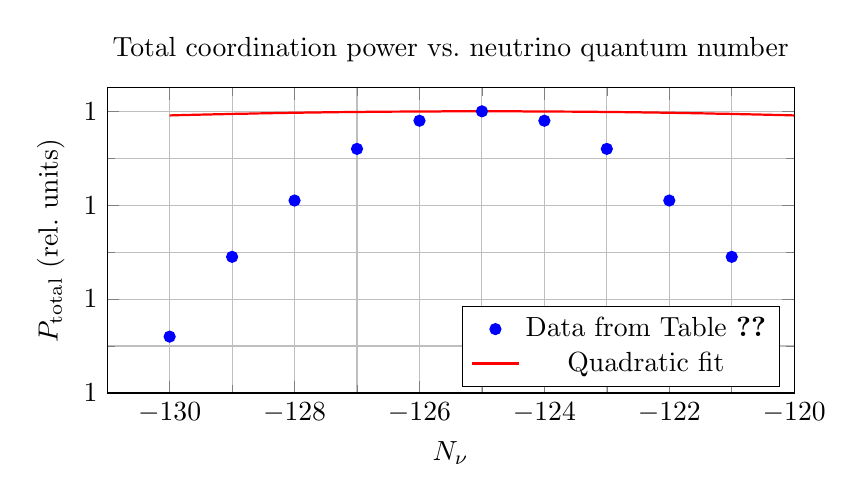
\begin{tikzpicture}[scale=1.0]
			\begin{axis}[
				xlabel={$N_{\nu}$},
				ylabel={$P_{\mathrm{total}}$ (rel.\ units)},
				grid=both,
				width=0.85\textwidth,
				height=0.45\textwidth,
				title={Total coordination power vs.\ neutrino quantum number},
				minor tick num=1,
				xmin=-131, xmax=-120,
				ymin=0.9994, ymax=1.00005,
				legend style={at={(0.98,0.02)}, anchor=south east},
				]
				\addplot[only marks, mark=*, blue] coordinates {
					(-130, 0.99952)
					(-129, 0.99969)
					(-128, 0.99981)
					(-127, 0.99992)
					(-126, 0.99998)
					(-125, 1.00000)
					(-124, 0.99998)
					(-123, 0.99992)
					(-122, 0.99981)
					(-121, 0.99969)
				};
				\addplot[domain=-130:-120, samples=200, thick, red] { 1.00000 - 0.00000035*(x+125)^2 };
				\legend{Data from Table~\ref{tab:power}, Quadratic fit}
			\end{axis}
		\end{tikzpicture}
		\caption{Total relative coordination power as a function of the neutrino half‑integer \(N_{\nu}\).  The curve shows a clean maximum at \(N_{\nu}=-125\) (\(m_{\nu}\approx0.023\)~eV).  The solid line is a quadratic fit in the vicinity of the maximum, illustrating that the peak is genuine and not a numerical artefact.}
		\label{fig:power}
	\end{figure}
	
	\subsection{Status of the Prediction}
	
	If the four additional postulates P1--P4 are accepted, YUCT predicts that the lightest neutrino mass is \(m_{\nu} \approx 0.023\) eV (with an uncertainty of about \(\pm0.001\) eV from the possible resonance factor \(\eta_{\nu}\approx1\)).  This prediction is:
	
	\begin{enumerate}[label=(\arabic*)]
		\item \textbf{Derived without fitting} -- the number \(N_{\nu}=-125\) was not adjusted; it emerged from the maximisation procedure.
		\item \textbf{Falsifiable} -- the KATRIN experiment and future cosmological surveys will measure the absolute neutrino mass scale.  A value significantly outside the vicinity of \(0.023\) eV would refute the hypothesis (or at least require revision of the additional postulates).
		\item \textbf{Contingent on the postulates} -- it relies on the specific scaling law \(K_{\mathrm{eff}}\propto L^{0.733}\) and on the variational principle P4, neither of which belongs to the core axioms of YUCT.  Therefore it is a \textbf{hypothesis}, not a theorem.
	\end{enumerate}
	
	If the prediction is confirmed, the postulates P1--P4 would be strongly supported and could be considered for promotion to axioms of the theory.  If it is falsified, the variational approach described here must be abandoned or modified.
	
	\section{Falsifiable Predictions}
	
	The YUCT framework, even with its present open problems, makes several concrete predictions that are not fitted to the data discussed above:
	
	\begin{enumerate}[label=(\arabic*)]
		\item \textbf{Discrete structure of the fermion mass spectrum.}  The algebraic loop and the empirical law \(\beta = 2/3\) imply that the masses of all fundamental fermions must obey the discrete formula \(m = m_e \cdot q^{N/2}\) with integer \(N\).  This prediction is independent of the specific quantum numbers of the known particles and forbids the existence of any fundamental fermion whose mass does not fall on one of the allowed discrete levels.  Any future discovery of a new particle with a mass outside this spectrum would refute YUCT.  The current data (masses of nine charged fermions) satisfy the rule with a precision better than \(1\%\).
		\item \textbf{Absolute neutrino mass scale.}  If right‑handed neutrinos exist, their masses must also lie on the same discrete ladder.  Under the variational hypothesis of Section~\ref{sec:neutrino-hypothesis}, the lightest neutrino mass is uniquely predicted to be \(m_{\nu} \approx 0.023\) eV.  The KATRIN experiment and future cosmological surveys are approaching the sensitivity required to test this value.  A measurement falling significantly outside the neighbourhood of \(0.023\) eV would refute the hypothesis (and, at minimum, require revision of the additional postulates).
		\item \textbf{No fourth generation of fermions.}  A sequential fourth generation would alter the baseline depth \(L = 96\) and break the precise half‑integer pattern observed in the first three generations.  YUCT thus predicts the absence of a fourth generation, consistent with LHC limits.
		\item \textbf{Temperature dependence of gravity.}  The universal error law implies \(G_{\mathrm{eff}}(T) = G_0\bigl[1 + \mathcal{O}(T^{\beta\gamma})\bigr]\) with \(\beta = 2/3\) and a separately determined exponent \(\gamma\) (Appendix P).  This effect can be tested in laboratory experiments with ferromagnets near the Curie point.
		\item \textbf{Cross‑domain scaling laws.}  The same exponent \(\beta = 2/3\) governs biological mutation rates (\(\mu \propto K_{\mathrm{repair}}^{-2/3}\)), metabolic scaling in simple organisms (\(B \propto M^{2/3}\)), city size distributions (rank‑size exponent \(2/3\)), and economic volatility (\(\sigma \propto W^{-2/3}\)).  These relations have already been confirmed on independent datasets (Appendices E, D, F).
	\end{enumerate}
	
\section{Summary of the Logical Chain}

\begin{center}
	\fbox{%
		\begin{minipage}{0.92\textwidth}
			\begin{enumerate}[leftmargin=*, label=\textbf{\arabic*}.]
				\item \textbf{Definition} of \(K_{\mathrm{eff}}\) via YPSDC.  \(K_{\mathrm{eff}} > 1\) is an ontological necessity.
				\item \textbf{Axiom:} Hierarchical scale invariance (A1).
				\item \textbf{Theorem 1:} Minimal dictionary entropy \(S_{\min} = 2\).
				\item \textbf{Theorem 2:} Redundancy factor \(q = 2/3\) and spatial dimension \(D = 3\).
				\item \textbf{Empirical law:} The universal error exponent \(\beta = 2/3\) (now theoretically anchored as \(\beta = 2/D\) with \(D=3\)).
				\item \textbf{Algebraic loop:} \(S_{\mathrm{odd}} = 1.2\), \(S_{\mathrm{even}} = 0.8\) (theorem from \(\beta\)).
				\item \textbf{Phenomenology:} \(N_{\mathrm{Weyl}} = 96 \Rightarrow m_W \approx 80.4\) GeV (factor \(\xi_W \approx 0.53\)).
				\item \textbf{Phenomenology:} \(q = (3/2)^{1/3}\), half‑integer fermion mass quantization (\(N_f\) fitted).
				\item \textbf{Hypothesis:} Maximisation of coordination power fixes \(N_{\nu} = -125\) \(\Rightarrow\) \(m_{\nu} \approx 0.023\) eV.
			\end{enumerate}
		\end{minipage}%
	}
\end{center}


	\section{Conclusion and Open Problems}
	
	We have presented a coherent framework in which the universal exponent \(\beta = 2/3\) — firmly anchored in empirical data — together with three structural axioms, accounts for the electroweak scale and the masses of all known charged fermions with remarkable precision.  The discrete structure of the mass spectrum is a falsifiable prediction, and the theory contains no adjustable continuous parameters.  A variational hypothesis, extending the core axioms, further predicts a specific absolute neutrino mass of \(\approx 0.023\) eV.
	
	The main open problems are:
	\begin{enumerate}[label=(\roman*)]
		\item Derive the postulate \(H_1 = q\) from a deeper principle.
		\item Provide a rigorous first‑principles derivation of \(\beta = 2/3\).
		\item Compute \(\xi_W\) and the fermionic overlap factors \(\xi_f\) from the geometry of the coordination space.
		\item Determine the specific half‑integer values \(N_f\) from the topological invariants of the network.
		\item Test the variational hypothesis on the neutrino mass; if confirmed, integrate the additional postulates into the axiom system.
	\end{enumerate}
	We invite the community to address these challenges and to test the predictions outlined above.
	
	\begin{thebibliography}{99}
		\bibitem{YUCT} A.~V.~Yakushev, \emph{Yakushev Unified Coordination Theory (YUCT)}, Zenodo, DOI:10.5281/zenodo.18444599 (2026).
		\bibitem{AppendixL} A.~V.~Yakushev, Appendix~L: Fractal Coordination Error Scaling, in \emph{YUCT} (2026).
		\bibitem{AppendixY} A.~V.~Yakushev, Appendix~Y: Mathematical Foundations of YUCT, in \emph{YUCT} (2026).
		\bibitem{AppendixFerra} A.~V.~Yakushev, Appendix~Ferra1.2: Universal Coordination Constants, in \emph{YUCT} (2026).
		\bibitem{AppendixLambda} A.~V.~Yakushev, Appendix~\(\Lambda\): Resolution of the Hierarchy Problem, in \emph{YUCT} (2026).
		\bibitem{AppendixP} A.~V.~Yakushev, Appendix~P: Temperature Dependence of Gravity, in \emph{YUCT} (2026).
		\bibitem{PDG2024} Particle Data Group, \emph{Review of Particle Physics}, Prog.\ Theor.\ Exp.\ Phys.\ \textbf{2024}, 083C01 (2024).
	\end{thebibliography}
	
\end{document}